\section{Základné pojmy}
Pred samotným uvedením do problému, ktorým sa zaoberá táto práca je dôležité vysvetliť a definovať základné pojmy, ktoré sú spojené s danou problematikou a využívané v texte. 

\subsection{Heslo}
Heslo je prostriedok, pomocou ktorého je overená totožnosť používateľa. \cite{1} Pomocou neho vieme získať prístup k informáciam, dátam atď. ktoré sú pod ním uzamknuté. Teda iba ten, kto heslo pozná, môže pristupovať k týmto materiálom. Z tohto môžeme usúdiť, že heslo by malo byť dostatočne silné. Musí byť ťažko uhádnuteľné a komplexné. Jeho vlastník by ho mal ukryť pred odhalením alebo uhádnutím útočníka. Týmto nám vznikajú rôzne otázky: \textit{Aké miesto je bezpečné na ukrytie hesla? Kedy môžeme prehlásiť, že heslo je "silné"?}

\subsection{Autentizácia}
\cite{2} Proces, pri ktorej je overená totožnosť osoby, sa nazýva autentizácia. Predchádza ju proces identifikácie, kedy sa osoba "predstaví" a povie, kto je. Systém ho ďalej v procese autentizácie "vyzve", aby dokázal, že dotyčná osoba je naozaj tou, za ktorú sa prehlásil. Tým dôkazom myslíme vyššie spomínané heslo.
	\par V praktickej rovine sú spôsoby autentizácie rôzne, ako napríklad: biometrický odtlačok, fráza vo forme hlasu, textového reťazca, číselný PIN a podobne \cite{3}. 

\subsection{Sila hesla} 
Uvažujme heslo ako textový reťazec. Sila hesla označuje stupeň obtiažnosti s akou ho neautorizovaná osoba dokáže uhádnuť \cite{4}. Heslo môže byť silné alebo slabé, v závislosti od toho, ako ťažké ho je uhádnuť \cite{4}. Slabé heslo je napríklad používanie iba malých písmen alebo iba číslic. Dôvod, prečo to tak je, je príliš malý priestor výberu znaku. Pri číselnom hesle hovoríme o priestore desiatich znakov. Uvažujme štandardnú telegrafnú abecedu s 26 písmenami. Potom je priestor pri použití hesla iba z malých písmen veľký 26 znakov. Útočník môže predpokladať, že používateľ má heslo zložené iba z číslic alebo iba z malých písmen\footnote{Možnosť použitia hesla iba z veľkých písmen nespomíname, pretože z matematického hľadiska náročnosti prelomenia hesla ide o rovnaký prípad ako pri malých písmenách.}. \par Preto na druhej strane hovoríme, že silné heslo je také heslo, ktoré obsahuje kombináciu veľkých a malých písmen a číslic. Už len kombináciou veľkých a malých písmen sa nám priestor zdvojnásobí. Abeceda veľkých písmen aj malých písmen má 26 znakov, čo je spolu 52 znakov. Zrazu je pre útočníka pri každom písmene nutné uvažovať, či sa použilo ako veľké, alebo ako malé. Z matematického hľadiska, teda z hľadiska permutácií sa celkový počet možných usporiadaní exponenciálne zvýši. Permutácia znamená usporiadanie.  


\begin{table}[ht]
\caption{Zložitosť prelomenia hesiel pomocou útoku brute-force}
\label{table:1}
\begin{tabular}{llll}
\textbf{Typ Hesla}        & \textbf{Heslo} & \textbf{Priestor} & \textbf{Počet možností} \\
Číslice (ďalej len C)     & 01234          & 10                & $1,11*10^5$             \\
Malé písmená (ďalej MP)   & heslo          & 26                & $1,24*10^7$             \\
MP + veľké písmená (VP)   & hEsLo          & 52                & $3,88*10^8$             \\
MP + VP + C               & h3sL0          & 62                & $9,31*10^8$             \\
MP + VP + C				  & h3sL0jeSiLn3   & 62				   & $3,28*10^{21}$			 \\
MP + VP + C + špec. znaky & h3sL0=\%SiLn3  & 95                & $5,46*10^{23}$           
\end{tabular}
\end{table}

\begin{table}[ht]
\begin{tabular}{ll}
\textbf{\begin{tabular}[c]{@{}l@{}}Čas (online útok)\\ pri 1000 pokusoch/s\end{tabular}} &
  \textbf{\begin{tabular}[c]{@{}l@{}}Čas (offline útok)\\ pri miliarde pokusoch/s\end{tabular}} \\
1,85 min            & 0,00000111 s \\
3,43 hod            & 0,000124 s   \\
4,49 dní            & 0,00388 s    \\
1,54 týždňov        & 0,00931 s    \\
104 miliárd rokov	& 1043 rokov   \\
17,4 biliónov rokov & 1740 rokov   \\
\end{tabular}
\end{table}

\par Z tabuľky sme pozorovaním zistili, že rovnako ako bohatý priestor znakov je dôležitá aj dĺžka hesla. S použitím veľkých aj malých písmen pri dĺžke hesla 5 by bol útočník schopný zistiť naše heslo za veľmi krátky čas. Môžeme si z časových výsledkov všimnúť, že z praktického hľadiska skoro ani nezáleží, či použijeme C, MP, MP + VP alebo MP + VP + C, pokiaľ je heslo krátke. Najmä pri offline útoku zjavne vidieť, že vo všetkých prípadoch by stroj uhádol heslo doslova do sekundy.
\par Silu exponenciálneho rastu si všímame pri zmene dĺžky hesla na 12 znakov. Celá situácia sa dramaticky zmenila a kombinácie C, MP a VP už dávajú zmysel. Ďalší veľký skok spôsobilo pridanie špeciálnych znakov. Keďže zväčšili priestor rôznych znakov o viac ako polovicu, významná zmena je vidieť aj vo výsledkoch.
\par \cite{5} Predpokladajme, že útočník má informáciu, že používateľ vlastní heslo zložené iba z MP. Potom platí, že ak by používateľ zväčšil dĺžku hesla o jeden znak, útočník musí vykonať v priemere o 26 viac pokusov pri každej permutácii.
\par \cite{5} Ďalej predpokladajme, že používateľ vlastní heslo zložené z MP, VP a C. Takáto kombinácia je dnes pri registrácii vo veľkej miere povinnosťou na rôznych webových stránkach. Potom platí, že pri zväčšení dĺžky hesla o jeden znak by sa zložitosť hesla nezvýšila iba 26, ale až 62-násobne. Z toho vyplýva, že útočník by musel mať 62-násobne väčší výkon, aby mohol za rovnaký čas zlomiť heslo z pôvodnou dĺžkou. Ten sa zvyšuje každé dva roky dvojnásobne, podľa Moorovho zákona. 
\newline \newline Táto úvaha spolu s ďalšími typmi útokov a ochranov pred nimi je hlbšie obsiahnutá v práci \cite{5}. 

\section{Problém password managerov}
Password manager ponúka používateľovi mnohé výhody. 


\section{Recitácia}
Citujem všetky zdroje v \textbf{bibliography.bib}, \cite{t00, t01, t02, t03, kniha, kniha2, kniha3, small, big, cs, koll, kap, tug, knuth, zbornik, prispevok}. \newline Good luck.
\section{Možnosti anonymizácie}
\noindent Anonymizácia znamená zmena alebo úprava údajov tak, aby sa podľa nich nedala jednoznačne určiť osoba, ktorej tieto údaje patria \cite{t01}. Existuje niekoľko spôsobov, ktorými môžeme dosiahnuť rôznu úroveň anonymizácie na internete: od mazania cookies súborov po ukončení prehliadania webových stránok až po používanie operačných systémov, ktoré sú na anonymite založené; od bezplatných možností až po komerčné verzie.  
\newline Nasleduje priblíženie niektorých možnosti anonymizácie.

\subsection{Súkromné prehliadanie}
\noindent Najpoužívanejšie internetové prehliadače súčasnosti majú v sebe zabudovanú funkcionalitu, ktorá dokáže čiastočne anonymizovať prístup na internet. Táto funkcionalita blokuje ukladanie navštívených stránok do histórie a nezaznamenáva súbory, ktoré sa stiahnu z~internetu. \acrshort{sw} a \acrlong{hw} sú skratky.

\begin{table}[!htbp]
\caption{Moduly a ich funkcie pri anonymizácii}
\label{modulyVlastnosti}
\begin{center}
\begin{tabular}{p{4cm}|c|c|c|c|c|c|c|c|c|c|c|c|c|c|c}
& \multicolumn{14}{c}%
	 {\textbf{Funkcia}}\\ \hline
&&&& & &\multicolumn{8}{c}%
	 {Modifikácia}\\ 
\textbf{Modul} &\begin{sideways} zobrazenie hlavičky \end{sideways} &\begin{sideways} blokovanie skriptov \end{sideways} &\begin{sideways} zmena IP \end{sideways} & \begin{sideways} zmena lokalizácie \end{sideways} & \begin{sideways} zmazanie/blokovanie cookies \end{sideways} & \begin{sideways} blokovanie trackerov \end{sideways}  & \begin{sideways} popis \end{sideways} & \begin{sideways}používateľský agent\end{sideways} & \begin{sideways} kódové označenie prehliadača \end{sideways} & \begin{sideways} názov prehliadača \end{sideways} & \begin{sideways} verzia prehliadača \end{sideways} & \begin{sideways} platforma \end{sideways} & \begin{sideways} výrobca prehliadača \end{sideways} & \begin{sideways} označenie výrobcu prehliadača \end{sideways} \\ \hline
User agent switcher & & & & & &  & X & X & X & X & X & X & X & X  \\ \hline
Ghostery &  && & & X & X &  &  & & & & & & \\  \hline
Better privacy && &  & & X &  &  &  & & & & & & \\  \hline
Anonymox &  && X & X & X &  & X & X & & & & & & \\  \hline
Modify headers & & &  &  & X &  &  & X &  &  &  & & &  \\  \hline
Request policy & & &  &  & & X  &  &  &  &  &  & & &   \\  \hline
Live HTTP headers & X& &  &  & &  &  &  &  &  &  & & &   \\  \hline
User agent awitcher for chrome & & &  &  & &  & X & X &  &  &  & & &   \\  \hline
Header hacker & & &  &  & &  & X & X & X & X & X & X & X & X    \\  \hline
Mod header & & &  &  & &  & X & X & X & X & X & X & X & X    \\  \hline
Script no & &X &  &  & &  &  &  &  &  &  &  &  &     \\  \hline
No script & &X &  &  & &  &  &  &  &  &  &  &  &     \\  \hline
Proxify it & & &X  & X & &  &  &  &  &  &  &  &  &     \\  \hline
I'm not here & & &  & X & &  &  &  &  &  &  &  &  &     \\  \hline
Get anonymous personal edition & &X &X &X &X&X &  &  &  &  &  &  &  &     \\  \hline
Anonymous browsing toolbar & & & X & X & &  &  &  &  &  &  &  &  &     \\  \hline
Easy hide your IP and surf anonymously & & & X & X& &  &  & X & X & X & X &  &  &     \\  \hline
\end{tabular}
\end{center}
\end{table}

\subsection{Anonymná sieť}
\noindent Anonymná sieť je sieť serverov, medzi ktorými dáta prechádzajú šifrované. V anonymných sieťach dáta prechádzajú z počítača používateľa, odkiaľ bola požiadavka poslaná, cez viaceré proxy smerovače, z ktorých každý správu doplní o smerovanie a zašifruje vlastným kľúčom. Cesta od ...


\subsection{Funkcionalita}
\noindent  Rozšírenie tiež okrem splnenia špecifikácie malo pre prehľadnosť a overenie funkčnosti zobrazovať údaje, ktoré boli na server odoslané. Zoznam údajov odoslaných na server, sa mal ukladať do krátkodobej histórie, aby nemal používateľ k dispozícií len najnovšie údaje, ale aj údaje odoslané v nejakom časovom období. Nejaky listing z priloh \ref{lst:sublime}.

\subsubsection{Funkcionalita2}
\noindent Samozrejmosťou bolo nastavenie zapnutia rozšírenia pri štarte, prípadne interval zmeny odosielaných údajov.

\subsection{Vzhľad}
\noindent Dôležitou požiadavkou kladenou na rozšírenie bolo príjemné používateľské rozhranie. Z~tohto dôvodu malo rozšírenie obsahovať zoznam modifikovaných vlastností a tlačidlo pre prístup k nastaveniam rozšírenia v jednoduchej a praktickej forme. Predpokladaný vzhľad je zobrazený na obrázku č. \ref{vzhladobr}.
\begin{figure}[!htbp]
  \centering
  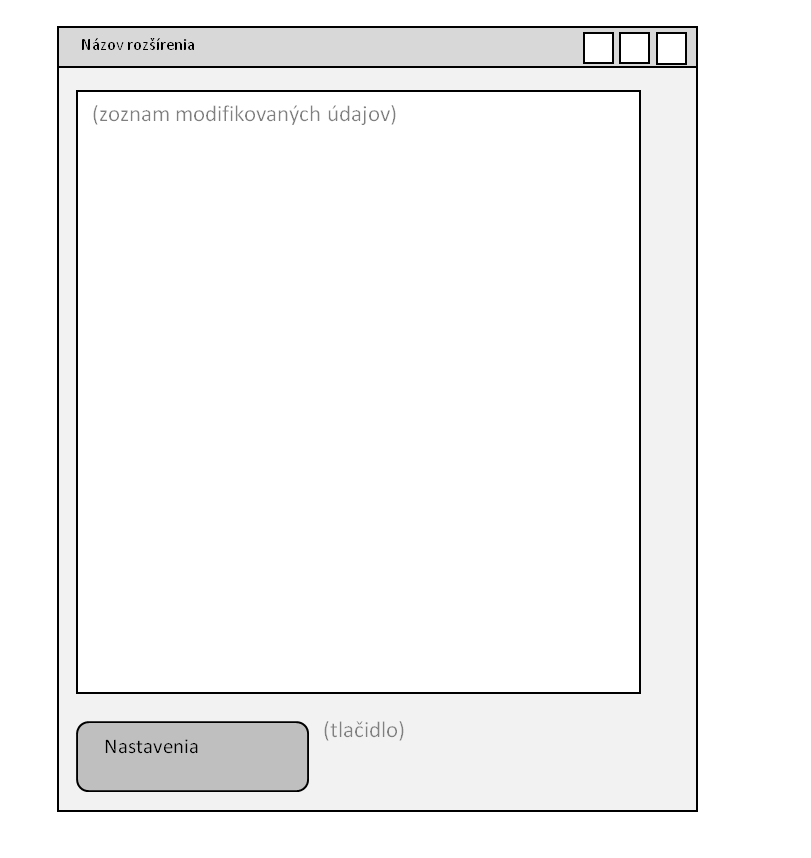
\includegraphics[width=8cm]{img/vzhlad.png}
  \caption{Predpokladaný vzhľad rozšírenia.}
  \label{vzhladobr}
\end{figure}	 
\noindent Dôležitou požiadavkou kladenou na rozšírenie bolo príjemné používateľské rozhranie.\cite{t00} Z~tohto dôvodu malo rozšírenie obsahovať zoznam modifikovaných vlastností a tlačidlo pre prístup k nastaveniam rozšírenia v jednoduchej a praktickej forme. Predpokladaný vzhľad je zobrazený na obrázku č. \ref{vzhladobr}.

\begin{algorithm}
\scriptsize
\begin{algorithmic}
 \STATE <text>
 \IF{<condition>} \STATE {<text>} \ELSE \STATE{<text>} \ENDIF
 \IF{<condition>} \STATE {<text>} \ELSIF{<condition>} \STATE{<text>} \ENDIF
 \FOR{<condition>} \STATE {<text>} \ENDFOR
 \FOR{<condition> \TO <condition> } \STATE {<text>} \ENDFOR
 \FORALL{<condition>} \STATE{<text>} \ENDFOR
 \WHILE{<condition>} \STATE{<text>} \ENDWHILE
 \REPEAT \STATE{<text>} \UNTIL{<condition>}
 \LOOP \STATE{<text>} \ENDLOOP
 \REQUIRE <text>
 \ENSURE <text>
 \RETURN <text>
 \PRINT <text>
 \COMMENT{<text>}
 \AND, \OR, \XOR, \NOT, \TO, \TRUE, \FALSE
\end{algorithmic}
\caption{Ukážka príkazov pre algorithmic}  
\label{alg:preview}  
\end{algorithm}

\begin{lstlisting}[
  caption={Ukážka algoritmu},
  label={lst:main-c},
  language=c
]
/* Hello World program */

#include<stdio.h>

struct cpu_info {
    long unsigned utime, ntime, stime, itime;
    long unsigned iowtime, irqtime, sirqtime;
};

main()
{
    printf("Hello World");
}
\end{lstlisting}